\documentclass{beamer}

\mode<presentation> {
\usetheme{Madrid}
}

\usepackage{graphicx} % Allows including images
\usepackage{booktabs} % Allows the use of \toprule, \midrule and \bottomrule in tables}
\usepackage{amsmath}
\usepackage{xcolor}
\usepackage{physics}
%----------------------------------------------------------------------------------------
%	TITLE PAGE
%----------------------------------------------------------------------------------------

\title[Wobbling Motion in odd-A nuclei]{A Novel Approach for the Semi-Classical Description of the Wobbling Properties in Odd-A Nuclei} % The short title appears at the bottom of every slide, the full title is only on the title page

\author{Robert Poenaru} % Your name
\institute[DFT] % Your institution as it will appear on the bottom of every slide, may be shorthand to save space
{
Department of Theoretical Physics, IFIN-HH \\
\vspace{0.1cm}
Faculty of Physics, University of Bucharest \\% Your institution for the title page
\medskip
\textit{robert.poenaru@drd.unibuc.ro} % Your email address
}
\date{\today} % Date, can be changed to a custom date

\begin{document}

\begin{frame}
\titlepage % Print the title page as the first slide
\end{frame}

\begin{frame}
\frametitle{Outline} % Table of contents slide, comment this block out to remove it
\tableofcontents % Throughout your presentation, if you choose to use \section{} and \subsection{} commands, these will automatically be printed on this slide as an overview of your presentation
\end{frame}


\section{Wobbling Motion} 

\begin{frame}{Nuclear shapes}
\begin{block}{Deformation parameters}
\begin{itemize}
    \item Nuclear shapes can be described via the \textbf{quadrupole parameter} $\beta$ and the \textbf{triaxiality parameter} $\gamma$.
\end{itemize}
\end{block}
\end{frame}

\begin{frame}{Triaxiality}
\begin{itemize}
    \item Nuclear shapes: most of the nuclei are spherical or axially symmetric in the ground state.
\end{itemize}
  \begin{figure}
    \centering
    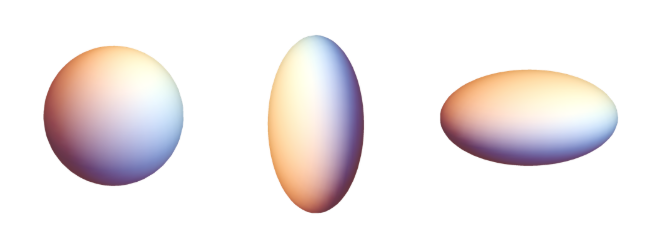
\includegraphics[scale=0.4]{figs/nuclear_shapes.png}
    \caption{\textbf{Spherical:} $\beta_2=0$ ; \textbf{Prolate:} $\beta_2>0$ ; \textbf{Oblate:} $\beta_2<0$}
  \end{figure}
\end{frame}


\begin{frame}
\frametitle{Multiple Columns}
\begin{columns}[c] % The "c" option specifies centered vertical alignment while the "t" option is used for top vertical alignment

\column{.45\textwidth} % Left column and width
\textbf{Heading}
\begin{enumerate}
\item Statement
\item Explanation
\item Example
\end{enumerate}

\column{.5\textwidth} % Right column and width
Lorem ipsum dolor sit amet, consectetur adipiscing elit. Integer lectus nisl, ultricies in feugiat rutrum, porttitor sit amet augue. Aliquam ut tortor mauris. Sed volutpat ante purus, quis accumsan dolor.

\end{columns}
\end{frame}

\begin{frame}
\frametitle{References}
\footnotesize{
\begin{thebibliography}{99} % Beamer does not support BibTeX so references must be inserted manually as below
\bibitem[Smith, 2012]{p1} John Smith (2012)
\newblock Title of the publication
\newblock \emph{Journal Name} 12(3), 45 -- 678.
\end{thebibliography}
}
\end{frame}

\begin{frame}
\Huge{\centerline{Thank you for your attention!}}
\end{frame}

\end{document} 